\documentclass[tikz,border=2mm]{standalone}
\usepackage{helvet}
\renewcommand{\familydefault}{\sfdefault}
\usetikzlibrary{arrows.meta,fit,positioning,calc}
\definecolor{datablue}{HTML}{4477AA}
\definecolor{methodteal}{HTML}{228833}
\definecolor{modelorange}{HTML}{CC6677}
\definecolor{uqgold}{HTML}{CC9933}
\definecolor{deploypurple}{HTML}{AA3377}
\definecolor{softgray}{HTML}{F2F2F2}
\begin{document}
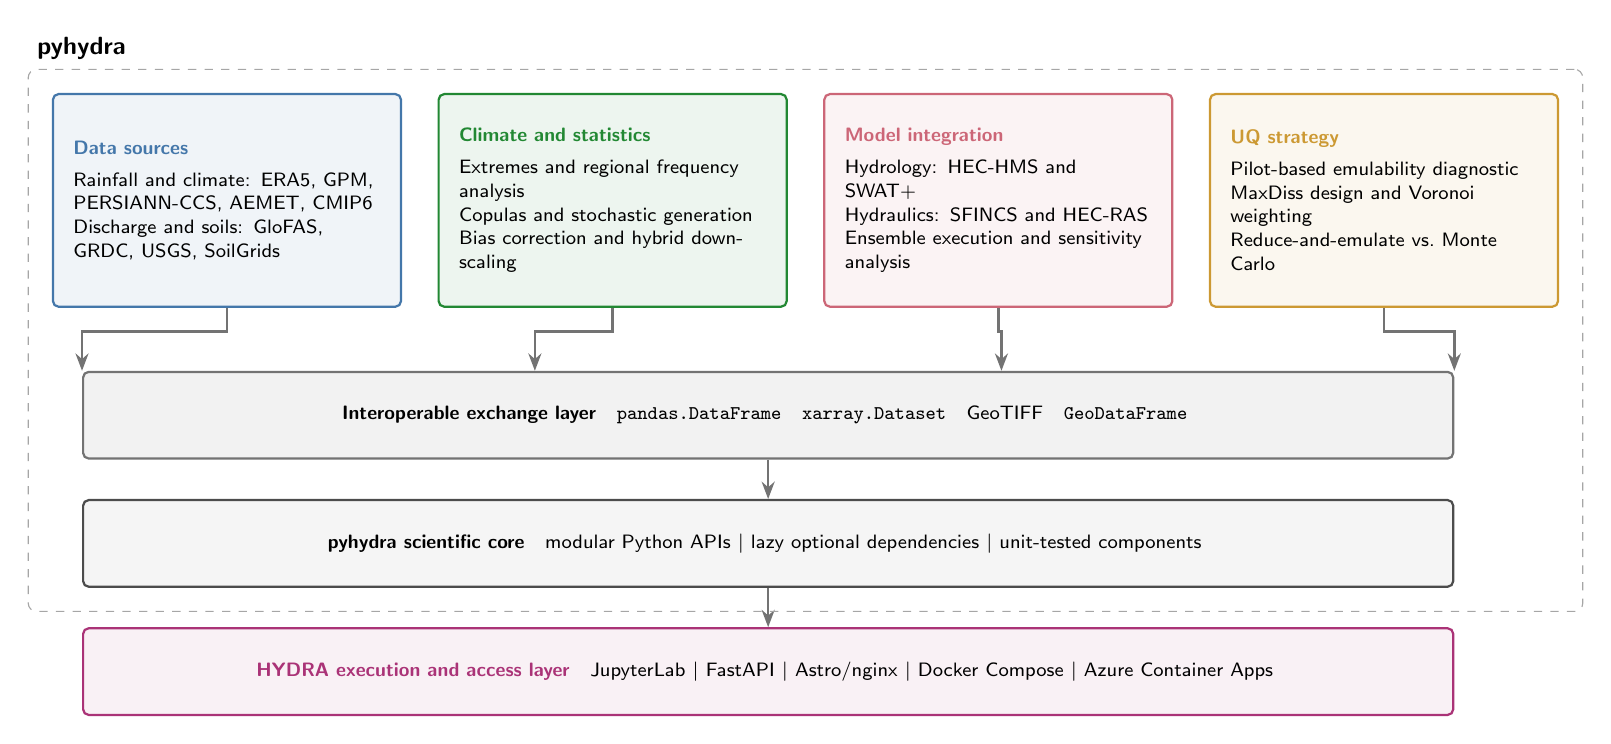
\begin{tikzpicture}[
  font=\fontsize{7.4}{8.6}\selectfont,
  title/.style={font=\bfseries\fontsize{9}{10.5}\selectfont},
  box/.style={rounded corners=2pt, line width=0.8pt, align=left,
    minimum height=27mm, text width=39mm, inner sep=2.6mm},
  layer/.style={rounded corners=2pt, line width=0.8pt, align=center,
    minimum width=174mm, minimum height=11mm, inner sep=2mm},
  arrow/.style={-{Stealth[length=2.2mm]}, line width=0.9pt, draw=black!55}
]
\node[box, draw=datablue, fill=datablue!8] (data) {
  \textbf{\color{datablue}Data sources}\\[1mm]
  Rainfall and climate: ERA5, GPM, PERSIANN-CCS, AEMET, CMIP6\\
  Discharge and soils: GloFAS, GRDC, USGS, SoilGrids
};
\node[box, draw=methodteal, fill=methodteal!8, right=4.5mm of data] (methods) {
  \textbf{\color{methodteal}Climate and statistics}\\[1mm]
  Extremes and regional frequency analysis\\
  Copulas and stochastic generation\\
  Bias correction and hybrid downscaling
};
\node[box, draw=modelorange, fill=modelorange!8, right=4.5mm of methods] (models) {
  \textbf{\color{modelorange}Model integration}\\[1mm]
  Hydrology: HEC-HMS and SWAT+\\
  Hydraulics: SFINCS and HEC-RAS\\
  Ensemble execution and sensitivity analysis
};
\node[box, draw=uqgold, fill=uqgold!8, right=4.5mm of models] (uq) {
  \textbf{\color{uqgold}UQ strategy}\\[1mm]
  Pilot-based emulability diagnostic\\
  MaxDiss design and Voronoi weighting\\
  Reduce-and-emulate vs.\ Monte Carlo
};

\node[layer, draw=black!55, fill=softgray, below=8mm of methods, xshift=19.75mm] (exchange) {
  \textbf{Interoperable exchange layer}\quad
  \texttt{pandas.DataFrame}\quad
  \texttt{xarray.Dataset}\quad
  GeoTIFF\quad
  \texttt{GeoDataFrame}
};
\node[layer, draw=black!70, fill=black!4, below=5mm of exchange] (core) {
  \textbf{pyhydra scientific core}\quad
  modular Python APIs $\mid$ lazy optional dependencies $\mid$ unit-tested components
};
\node[layer, draw=deploypurple, fill=deploypurple!7, below=5mm of core] (hydra) {
  \textbf{\color{deploypurple}HYDRA execution and access layer}\quad
  JupyterLab $\mid$ FastAPI $\mid$ Astro/nginx $\mid$ Docker Compose $\mid$ Azure Container Apps
};

\draw[arrow] (data.south) -- ++(0,-3mm) -| (exchange.north west);
\draw[arrow] (methods.south) -- ++(0,-3mm) -| ($(exchange.north west)!0.33!(exchange.north east)$);
\draw[arrow] (models.south) -- ++(0,-3mm) -| ($(exchange.north west)!0.67!(exchange.north east)$);
\draw[arrow] (uq.south) -- ++(0,-3mm) -| (exchange.north east);
\draw[arrow] (exchange) -- (core);
\draw[arrow] (core) -- (hydra);

\node[fit=(data)(methods)(models)(uq)(exchange)(core), inner sep=3mm,
  draw=black!35, dashed, rounded corners=3pt,
  label={[title,anchor=south west]north west:pyhydra}] {};
\end{tikzpicture}
\end{document}
